% Mo Jabeen Template for docs 

\documentclass[11pt]{scrartcl} % Font size

%%%%%%%%%%%%%%%%%%%%%%%%%%%%%%%%%%%%%%%%%
% Wenneker Assignment
% Structure Specification File
% Version 2.0 (12/1/2019)
%
% This template originates from:
% http://www.LaTeXTemplates.com
%
% Authors:
% Vel (vel@LaTeXTemplates.com)
% Frits Wenneker
%
% License:
% CC BY-NC-SA 3.0 (http://creativecommons.org/licenses/by-nc-sa/3.0/)
% 
%%%%%%%%%%%%%%%%%%%%%%%%%%%%%%%%%%%%%%%%%

%----------------------------------------------------------------------------------------
%	PACKAGES AND OTHER DOCUMENT CONFIGURATIONS
%----------------------------------------------------------------------------------------

\usepackage{amsmath, amsfonts, amsthm} % Math packages

\usepackage{listings} % Code listings, with syntax highlighting

\usepackage[english]{babel} % English language hyphenation

\usepackage{graphicx} % Required for inserting images
\graphicspath{{Figures/}{./}} % Specifies where to look for included images (trailing slash required)

\usepackage{booktabs} % Required for better horizontal rules in tables

\numberwithin{equation}{section} % Number equations within sections (i.e. 1.1, 1.2, 2.1, 2.2 instead of 1, 2, 3, 4)
\numberwithin{figure}{section} % Number figures within sections (i.e. 1.1, 1.2, 2.1, 2.2 instead of 1, 2, 3, 4)
\numberwithin{table}{section} % Number tables within sections (i.e. 1.1, 1.2, 2.1, 2.2 instead of 1, 2, 3, 4)

\setlength\parindent{0pt} % Removes all indentation from paragraphs

\usepackage{enumitem} % Required for list customisation
\setlist{noitemsep} % No spacing between list items

\usepackage{array}
\newcolumntype{P}[1]{>{\centering\arraybackslash}p{#1}} %Allows centering of tables

\usepackage[
backend=biber,
style=ieee,
sorting=ynt
]{biblatex}

\addbibresource{refs.bib} %Imports bibliography file

%----------------------------------------------------------------------------------------
%	DOCUMENT MARGINS
%----------------------------------------------------------------------------------------

\usepackage{geometry} % Required for adjusting page dimensions and margins

\geometry{
	paper=a4paper, % Paper size, change to letterpaper for US letter size
	top=2.5cm, % Top margin
	bottom=3cm, % Bottom margin
	left=3cm, % Left margin
	right=3cm, % Right margin
	headheight=0.75cm, % Header height
	footskip=1.5cm, % Space from the bottom margin to the baseline of the footer
	headsep=0.75cm, % Space from the top margin to the baseline of the header
	%showframe, % Uncomment to show how the type block is set on the page
}

%----------------------------------------------------------------------------------------
%	FONTS
%----------------------------------------------------------------------------------------

\usepackage[utf8]{inputenc} % Required for inputting international characters
\usepackage[T1]{fontenc} % Use 8-bit encoding

\usepackage{fourier} % Use the Adobe Utopia font for the document

%----------------------------------------------------------------------------------------
%	HEADERS AND FOOTERS
%----------------------------------------------------------------------------------------

\usepackage{scrlayer-scrpage} % Required for customising headers and footers

\ohead*{} % Right header
\ihead*{} % Left header
\chead*{} % Centre header

\ofoot*{} % Right footer
\ifoot*{} % Left footer
\cfoot*{\pagemark} % Centre footer

%----------------------------------------------------------------------------------------
%	SECTION TITLES
%----------------------------------------------------------------------------------------
 % Include the file specifying the document structure and custom commands

%----------------------------------------------------------------------------------------
%	TITLE SECTION
%----------------------------------------------------------------------------------------

\title{	
	\normalfont\normalsize
	\vspace{20pt} % Whitespace
	{\huge KiCAD Cheat Sheet}\\ % The meh
	\vspace{12pt} % Whitespace
	\rule{\linewidth}{2pt}\\ % Thick bottom horizontal rule
}

\author{\small Dainish Jabeen} % Your name

\date{\normalsize\today} % Today's date (\today) or a custom date

\begin{document}

\maketitle % Print the title

\section{KiCAD}

KiCAD is designed to:
\begin{itemize}
	\item Create circuit schematics
	\item Create PCBs
\end{itemize}

To ensure functioning PCBs are created, KiCAD offers the following:
\begin{itemize}
	\item PCB Calculator (Determine electrical component properties)
	\item Gerber viewer (inspect manufacturing files)
	\item 3D viewer
	\item Integrated SPICE simulation
\end{itemize}

KiCAD has a manual workflow of first building the schematic then completing the PCB layout.\\

4 Base programs:
\begin{itemize}
	\item Schematic editor
	\item PCB editor
	\item Symbol editor
	\item Footprint editor
\end{itemize}

\textbf{First step is to create a project, which has connected files for schematic and PC.}

\section{Tips}

\begin{itemize}
	\item R: rotate object
	\item G: move object with wires attached
	\item M: move object without wires
	\item U: select multi traces connecting components
\end{itemize}

\section{Create a schematic}

\begin{enumerate}
	\item In page setting give a title and rev number.
	\item Use under lined A for any additional labelling
	\item Choose component values (E: properties)
	\begin{itemize}
		\item Comp val: Manufacturers part number
	\end{itemize}
	\item Choose Footprint for each item (E)
	\item Run ERC
	\begin{itemize}
		\item Power symbols (power flag) are required to power output pins (VCC, GND)
	\end{itemize}
	\item Create BOM
\end{enumerate}

\section{Create a PCB}

The appearance panel on the right is for controlling the layers.

\begin{enumerate}
	\item Setup page (page settings)
	\item Setup board 
	\begin{itemize}
		\item Physical stackup (number of layers)
		\item Constraints: Should match the fab house
		\item Can have different constraints for different fab house
	\end{itemize}
	\item Update from schematic
	\item Draw board outline (layer Edge cuts)
	\item Place comps
	\begin{itemize}
		\item F: Flip to other side of board
	\end{itemize}
	\item Route tracks
	\begin{itemize}
		\item F.Cu : Front
		\item B.Cu : Back
		\item V: Insert via
	\end{itemize}
	\item Copper zones
	\begin{itemize}
		\item Draw zone (should be slightly bigger than board)
		\item Fill all zones (has to be done manually after changes, use B)
	\end{itemize}
	\item Design rule check
	\item 3D viewer
	\item Fab output (Plot + Drill files)
\end{enumerate}

\section{Create custom symbol}

\begin{enumerate}
	\item Create new global symbol library (Symbol editor -> new library)
	\item Create symbol in lib
	\begin{itemize}
		\item Add pins
		\item Switch grid size to make changes easier
	\end{itemize}
	\item Set symbol properties (double click on page)
	\begin{itemize}
		\item Set keywords for easy find
	\end{itemize}
	\item Create footprint via footprint editor (of components physical object)
	\begin{itemize}
		\item Pin 1 is normally placed at 0,0
	\end{itemize}
	\item Add pads
	\begin{itemize}
		\item Add margin for diameter and pads
	\end{itemize}
	\item Add outline
	\begin{itemize}
		\item Fab layer
		\item Silkscreen layer
		\item Courtyard
		\item \[ silkscreen\;margin = fab_width/2 + silk_width/2 \] 
	\end{itemize}
	\item Link footprint to symbol
\end{enumerate}

\section{SPICE Simulation}

Simulation program with integrated circuit emphasis.\\

Example statement: .[type] [step time] [fixed time] i.e. .tran 1u 1m

\begin{itemize}
	\item SPICE uses component sim models (.lib files) to describe the behavior of components.
	\item Simple components (resistor and capacitor) models are auto assigned, others need to be manually assigned.
	\item \textbf{KiCAD and sim model may use different pins}
	\item Placing SPICE statements as text, allows them to be saved
	\item Set compatibility to PSPICE and LTSPICE
	\item Use labels to read probe sim values easier
	\item Netlist shows connections in sim
	\item \#branch: shows the current
	\item Show cursor on signal list to see val over time
\end{itemize}

Use global power ref points with SPICE power components \ref{Power comp}, to simulate voltages. VSIN is for variable
voltage waveform. 

\begin{figure}[h] % [h] forces the figure to be output where it is defined in the code (it suppresses floating)
	\centering
	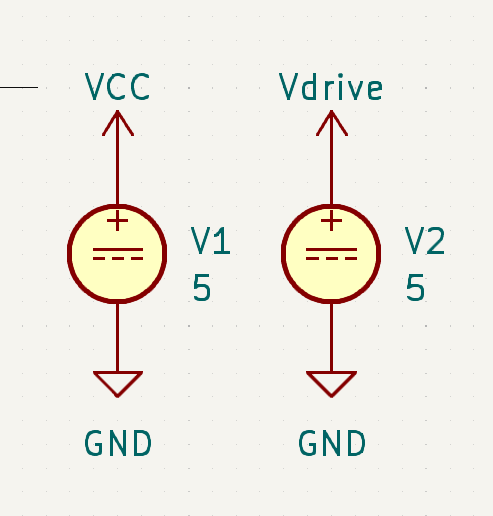
\includegraphics[width=0.5\columnwidth]{power comp.png} % Example image
	\caption{Power comp ref}
	\label{Power comp}
\end{figure}

%----------------------------------------------------------------------------------------
%	FIGURE EXAMPLE
%----------------------------------------------------------------------------------------

% \begin{figure}[h] % [h] forces the figure to be output where it is defined in the code (it suppresses floating)
% 	\centering
% 	\includegraphics[width=0.5\columnwidth]{IMAGE_NAME.jpg} % Example image
% 	\caption{European swallow.}
% \end{figure}

%----------------------------------------------------------------------------------------
% MATH EXAMPLES
%----------------------------------------------------------------------------------------

% \begin{align} 
% 	\label{eq:bayes}
% 	\begin{split}
% 		P(A|B) = \frac{P(B|A)P(A)}{P(B)}
% 	\end{split}					
% \end{align}

%----------------------------------------------------------------------------------------
%	LIST EXAMPLES
%----------------------------------------------------------------------------------------

% \begin{itemize}
% 	\item First item in a list 
% 		\begin{itemize}
% 		\item First item in a list 
% 			\begin{itemize}
% 			\item First item in a list 
% 			\item Second item in a list 
% 			\end{itemize}
% 		\item Second item in a list 
% 		\end{itemize}
% 	\item Second item in a list 
% \end{itemize}

%------------------------------------------------

% \subsection{Numbered List}

% \begin{enumerate}
% 	\item First item in a list 
% 	\item Second item in a list 
% 	\item Third item in a list
% \end{enumerate}

%----------------------------------------------------------------------------------------
%	TABLE EXAMPLE
%----------------------------------------------------------------------------------------

% \section{Interpreting a Table}

% \begin{table}[h] % [h] forces the table to be output where it is defined in the code (it suppresses floating)
% 	\centering % Centre the table
% 	\begin{tabular}{l l l}
% 		\toprule
% 		\textit{Per 50g} & \textbf{Pork} & \textbf{Soy} \\
% 		\midrule
% 		Energy & 760kJ & 538kJ\\
% 		Protein & 7.0g & 9.3g\\
% 		\bottomrule
% 	\end{tabular}
% 	\caption{Sausage nutrition.}
% \end{table}

%----------------------------------------------------------------------------------------
%	CODE LISTING EXAMPLE
%----------------------------------------------------------------------------------------

% \begin{lstlisting}[
% 	caption= Macro definition, % Caption above the listing
% 	language=python, % Use Julia functions/syntax highlighting
% 	frame=single, % Frame around the code listing
% 	showstringspaces=false, % Don't put marks in string spaces
% 	numbers=left, % Line numbers on left
% 	numberstyle=\large, % Line numbers styling
% 	]

% 	CODE

% \end{lstlisting}

%----------------------------------------------------------------------------------------
%	CODE LISTING FILE EXAMPLE
%----------------------------------------------------------------------------------------

% \lstinputlisting[
% 	caption=Luftballons Perl Script., % Caption above the listing
% 	label=lst:luftballons, % Label for referencing this listing
% 	language=Perl, % Use Perl functions/syntax highlighting
% 	frame=single, % Frame around the code listing
% 	showstringspaces=false, % Don't put marks in string spaces
% 	numbers=left, % Line numbers on left
% 	numberstyle=\tiny, % Line numbers styling
% 	]{luftballons.pl}

%----------------------------------------------------------------------------------------
%	BIB EXAMPLE
%----------------------------------------------------------------------------------------

% Using \texttt{biblatex} you can display a bibliography divided into sections, depending on citation type. 
% Let's cite! Einstein's journal paper \cite{einstein} and Dirac's book \cite{dirac} are physics-related items. 
% Next, \textit{The \LaTeX\ Companion} book \cite{latexcompanion}, Donald Knuth's website \cite{knuthwebsite}, \textit{The Comprehensive Tex Archive Network} (CTAN) \cite{ctan} are \LaTeX-related items; but the others, Donald Knuth's items, \cite{knuth-fa,knuth-acp} are dedicated to programming. 

% \medskip

% \printbibliography[
% heading=bibintoc,
% title={Whole bibliography}
% ] %Prints the entire bibliography with the title "Whole bibliography"

% %Filters bibliography
% \printbibliography[heading=subbibintoc,type=article,title={Articles only}]
% \printbibliography[type=book,title={Books only}]

% \printbibliography[keyword={physics},title={Physics-related only}]
% \printbibliography[keyword={latex},title={\LaTeX-related only}]

\end{document}